\documentclass[12pt,english]{amsart}
%\usepackage[margin=0.5in]{geometry}
\usepackage[a4paper, margin=2cm]{geometry}
\linespread{1.5}

%\usepackage{fontspec}
%\setmainfont{Times New Roman}
\usepackage{mathptmx}

\usepackage{graphicx}
\usepackage{wrapfig}
\usepackage{lscape}
\usepackage{rotating}
\usepackage{epstopdf}

\usepackage{verbatim}
\usepackage{url}
\usepackage{xspace}

\usepackage{listings}
\usepackage{color}
    \definecolor{light}{gray}{0.97}
    \definecolor{dark}{gray}{0.30}
\lstset{
%columns=fullflexible,
%basicstyle=\ttfamily,
escapeinside={||},
    %mathescape=true,
    language=C, % choose the language of the code
    basicstyle=\fontfamily{pcr}\selectfont\scriptsize\color{black},
    keywordstyle=\color{black}\bfseries, % style for keywords
    numbers=none, % where to put the line-numbers
    numberstyle=\tiny, % the size of the fonts that are used for the line-numbers
    backgroundcolor=\color{light},
    showspaces=false, % show spaces adding particular underscores
    showstringspaces=false, % underline spaces within strings
    showtabs=false, % show tabs within strings adding particular underscores
    %frame=single, % adds a frame around the code
    tabsize=2, % sets default tabsize to 2 spaces
    %rulesepcolor=\color{gray}
    captionpos=b, % sets the caption-position to bottom
    breaklines=false, % sets automatic line breaking
    %breakatwhitespace=false,
    numbersep=2em,
    % C was used in the blocksworld example to refer to block C and nowhere else
    emph={par,or,hor,do,end,loop,code,await,pause,emit,input,event,call,with,%
          var,and,then,else,return,pure,deterministic,nohold,finalize,%
          class, every, FOREVER, this, spawn, in, pool, watching, until, 
          interface, each, abort, when, signal, PROC, CHAN, SIGNAL, PAR, not,
          bool, tag, escape, traverse,implementation,output,true,false,
          native,@const,@pure,@safe,define,public,private,none},
    emphstyle={\bfseries},
    commentstyle=\color{dark}\scriptsize,
    %xleftmargin=20pt,
    %xrightmargin=20pt,
    framesep=20pt,
    %upquote=true,
    %aboveskip={1.5\baselineskip},
}

\newcommand{\CEU}{\textsc{C\'{e}u}\xspace}
\newcommand{\code}[1] {{\small{\texttt{#1}}}}

\usepackage{enumitem}
\setlist{nolistsep}

% Auto-Standby
\title{Energy Efficiency for IoT Software in the Large \\ Progress Report}

\author{Francisco Sant'Anna, UERJ}

\begin{document}

%\date{\today}
\maketitle

\vspace{-0.5cm}
%\newpage

\section{Original Proposal}

Considering the projected scale of the IoT for the next decade and the role of
low-power standby towards energy efficiency~\cite{iea.data}, this research
project has the following goals:

\begin{enumerate}
    \item Address energy efficiency through rigorous use of standby.
    \item Target constrained embedded architectures that form the IoT.
    \item Provide standby mechanisms at the programming language level that
          scale to all applications.
    \item Support transparent/non-intrusive standby mechanisms that reduce
          barriers of adoption.
\end{enumerate}

This proposal lies at the bottom of the software development
layers---transparent programming language mechanisms---meaning that \emph{all}
applications would take advantage of low-power standby modes automatically,
without extra programming efforts.
%
We expect that existing energy-unaware applications will benefit from savings
in the order of 50\%.
%
We will require a budget of R\$70k:
R\$60k to support three students, R\$5k for equipment, and
R\$5k for publication and travel costs.

The bulk of this proposal is grounded on the design of \CEU~\cite{ceu.tecs17},
a new reactive programming language targeting resource-constrained embedded
systems, which I have been working for the past 8 years.
%
The language is grounded on the synchronous concurrency model, which trades
power for reliability and has a simpler model of time that suits most
requirements of IoT applications.
%
In this model, all reactions to the external world are guaranteed to be
computed in bounded time, ensuring that applications always reach an idle state
amenable to standby mode.

\section{Timeline of Main Events}

\begin{description}
\item[Jul/17]
    Early explorations with the core idea of the project.
\item[Sep/17]
    Submission of the proposal to Serrapilheira.
\item[Dec/17]
    Grant award notification from Serrapilheira.
\item[Jan/18]
    Submission of two student scholarships to \emph{Google Summer of Code (GSoC'18)}%
    \footnote{\emph{GSoC'18}: \url{https://summerofcode.withgoogle.com/}}.
\item[Fev/18]
    First fully-working prototype of \CEU with support for interrupts and a
    power manager.
\item[Fev/18]
    Submission to \emph{LCTES'18} %
    \footnote {
        \emph{19th Annual ACM SIGPLAN / SIGBED Conference on Languages,
            Compilers, and Tools for Embedded Systems}:
        \url{https://conf.researchr.org/track/LCTES-2018/LCTES-2018-papers}.
    }
    of a work-in-progress paper entitled \emph{``Transparent Standby for
    Low-Power, Resource-Constrained Embedded Systems: A Programming
    Language-Based Approach''}~\cite{ceu.lctes18.short} and a full paper entitled \emph{``A
    Memory-Bounded, Deterministic and Terminating Semantics for the Synchronous
    Programming Language \CEU''}~\cite{ceu.lctes18}.
\item[Mar/18]
    Admission into the graduate program of Electrical Engineering at UERJ.
    \\
    Invitation to be program chair of \emph{REBLS'18} %
    \footnote {
        \emph{5th ACM SIGPLAN Workshop on Reactive and Event-based Languages \& Systems}:
        \url{https://2018.splashcon.org/track/rebls-2018-papers}.
    }.
\item[Mar-May/18]
    Engineering efforts on the prototype: refactoring, optimizations, more
    drivers, multiple platforms (AVR \& SAMD).
\item[Apr/18]
    Grant agreement signature with Serrapilheira.
    \\
    Grant award notification from Google for the two \emph{GSoC'18} students%
    \footnote{\emph{LabLua@GSoC'18}: \url{https://summerofcode.withgoogle.com/organizations/5641514328260608/}}:
    Anny (from UERJ) will work on a integrated programming environment for \CEU.
    Naveen (from India) will work on new device drivers.
\item[Apr/18]
    First full-application experiments with significant energy savings ranging
    from 20-99\%.
\item[Jun/18]
    Admission of Anna (from PUC-Rio) as an intern to work on new IoT
    applications.
\item[Jun/18]
    Trip to present the two papers on \emph{LCTES'18}.
\end{description}

\section{Progress Report}

Since the grant notification at the end of last year, our main goal was to
reach, as fast as possible, a working prototype of our core research idea.
%
I worked towards a new version of our programming language \CEU that would
provide automatic standby for all applications:
    a programmer writes an IoT application unaware of standby or energy
    constraints and the language puts the device to sleep whenever possible.

In parallel, I worked with colleagues from PUC-Rio on a formal semantics of
\CEU and a proof that all valid programs will react to an external event in
bounded time, with bounded memory, and deterministic behavior.
This proof is an important result because it shows that applications always
reach an idle state amenable to standby.
The formalization of \CEU already appeared on my PhD thesis~\cite{ceu.phd}, but
the proofs are new results from this year.

By the end of February was the submission deadline for \emph{LCTES'18}, the
main annual venue that links programming languages and embedded systems.
Fortunately, we had enough time to submit a full paper with the
proofs~\cite{ceu.lctes18} and a work-in-progress paper describing our approach
for transparent standby at the language level~\cite{ceu.lctes18.short}, both
of which were accepted for publication.
%
Even though we did not have a comprehensive evaluation of energy savings, the
conceptual framework and working prototype raised enough interest in the
community for discussion on the conference.

\begin{figure}
\begin{minipage}{0.35\textwidth}
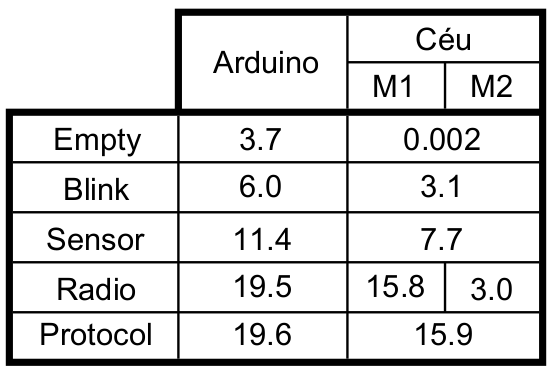
\includegraphics[width=\linewidth]{results3}
\end{minipage}
\begin{minipage}{0.33\textwidth}
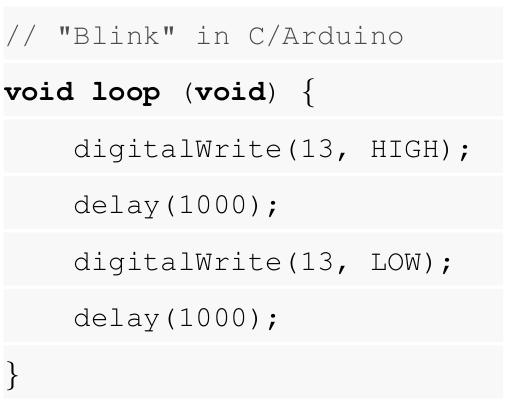
\includegraphics[width=\linewidth]{blink_c}
\end{minipage}
\begin{minipage}{0.28\textwidth}
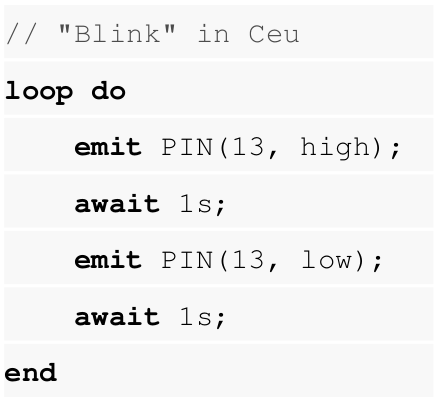
\includegraphics[width=\linewidth]{blink_ceu}
\end{minipage}
\caption{ Energy consumption for 5 scenarios.
          ``Blink'' in C/Arduino and \CEU.
\label{lst.eval}
}
\end{figure}

At this moment, we have more concrete evaluation scenarios that show
significant reduction in energy consumption due to standby in the
microcontroller and other peripherals.
%
Figure~\ref{lst.eval} shows the energy consumption of five applications
originally in C/Arduino which we rewrote in \CEU.
%
The first case illustrates how a naive ``Empty'' application in C/Arduino
remains 100\% of the time awake while the same application in \CEU sleeps in
the most efficient standby mode.
%
The ``Blink'' example shows that \CEU preserves the sequential, easy-to-read
style of C/Arduino, while consuming much less energy.
This is due to the assumptions \CEU, based on its tractable semantics, can
extract from the program to be sure that it can sleep on the calls to
\code{await}.
%
The ``Radio'' example is another interesting case because the radio driver in
\CEU identifies that the radio peripheral can enter in sleep mode to consume
much less energy (toggling between active and passive radio modes).

Considering the second phase to come and the interactions with Serrapilheira
since the beginning of the first phase and, it became more and more clear that
the grant evaluation criteria will be mostly based on long-term relevance of
the research and that it will encourage more fundamental aspects.
%
In this direction, we chose to invest considerable efforts on the foundations
of the language, highlighting its distinguished semantic aspects that enable
transparent standby.
The paper with the termination proof is the first result in this front, and we
want to continue in this direction by employing automatic verification tools,
such as TODO.
More concretely, we want to automate the manual proofs we currently have and
also answer program specification questions such as "Can we prove that this
application will turn off the radio 10 minutes after receiving a certain
message?"
%
Another education
%
At the beginning of this year I was invited to be the program of
\emph{REBLS'18} which is
The REBLS fundamentals of reactive languages
foundational models of reactive languages


Specification correctness

Dafny is a verification-aware programming language
    - program verifier

LiquidHaskell
 logical predicates that let you enforce critical properties at compile time
    - Avoid Infinite Loops
    - Enforce Correctness Properties
    - Prove Laws by Writing Code

REBLS is about the future of our area

How IoT development will affect the new generation and how our undergraduate
courses are ready to .


- new results
- education: IoT and Cyber physical strong on graduate, not 
    - lack of accessible languages and concurrency programming environments
    - specially energy efficiency

- incluir o standby de componentes na avaliacao
- mostrar o que nao dá pra fazer com TinyOS
    - como seria o caso de par/or em que o finalize remove o periferico da lista de possiveis awakes?
    - e o caso de componentes que são inteiramente desligados
        - caso de um par/or que mata o
            - radio listening
            - o radio inteiramente
        - como desligar dentro de finalize coisas que são desligadas via emit/await?


questions such as, can I prove that this particular program will


My initial budget plan was to spend around R\$5k per month with research staff
(80\% of the budget).
In particular, we wanted a professional embedded system engineer early in the
project full time on the heavy-lifting work on drivers and platforms to serve
as basis for for developing IoT applications.
%
However, since the grant became available only on April, I could not hire such
professional.
%
Nonetheless, I could dedicate most of my time until May on the engineering
aspects of the project, since the core language mechanisms were developed
between December and February.
At the end, the outcome was actually favorable since I overestimated the
importance of an experienced domain-specific engineer at an early stage.
The saved money was redirected to the international trip which was not
initially planned.

Another difficulty that we had to deal was the lack of students to work in the
area of embedded systems, even when offering above-average remuneration.
%
Furthermore, as a new professor in my University I was not associated with any
graduate program until mid March, when I joined the Electrical Engineering
program in the field of \emph{Networks \& Distributed Systems}.
However, we currently only offer Master degrees and most of the students have
part-time commitment with the program.
%
The scholarships from Google for \emph{GSoC'18} raise more interest on students
and we could hire an undergraduate student that is working 


part time

(Doctorate degrees

the University currently has no Doctorate program with 


On April we were notified about two scholarships 




%
My current plan is 

Another



porting 
SAMD
From the very beginning, 




the concept


describing the 

all programs 

Céu is a synchronous programming language for embedded soft real-time systems. It focuses on control-flow safety features, such as safe shared-memory concurrency and safe abortion of lines of execution, while enforcing memory bounded, deterministic, and terminating reactions to the environment.
In this work, we present a small-step structural operational semantics for Céu

 and a proof that reactions have the properties enumerated above: that for a given arbitrary timeline of input events, multiple executions of the same program always react in bounded time and arrive at the same final finite memory state.

By the end of February

- Theoretical
- Core
- Engineering
- Experiments

\begin{comment}
- Include a working title and the words "Progress Report" at the top of the page.
- Use section headings in the report to simplify both the writing and reading process.
- Open the report with a "Scope and Purpose" section, where you give a condensed version of your future report’s introduction and objective.
- Always include a section entitled, for example, "Progress," which summarizes the work’s pace and progress and explains any snafus, dilemmas, or setbacks.
- Always include a section entitled, for example, "Remaining Work," which honestly assesses the work that must still be completed. Think right on the page in this section, posing questions, speculating meaningfully, exploring your options.
- Always include a section that projects the expected results. Commit to a schedule for obtaining those results if possible.
- If necessary, include a section in which you directly solicit advice from your teacher or advisor. Be forthright and professional about the nature of the advice you need.
- Keep your paragraphs short and focused—just a few paragraphs per section, typically.
- Your tone can often be straightforward and familiar—therefore, as a rule, you can use "I" and "you" freely—but do not lapse into informality.
- Avoid being overly optimistic, pessimistic, apologetic, cocky, or self-deprecating.
\end{comment}

\bibliographystyle{abbrv}
\bibliography{serra,my}
\end{document}
